\section{Development method}

Development Method
There are many development methods, and we prefer the conventional method it is Waterfall. The waterfall model can work if everything goes to plan, but in a complex project things rarely do. The core of the problem is the reliance on getting the specification perfect before attempting to it.

\begin{figure}[h]
	\centering
	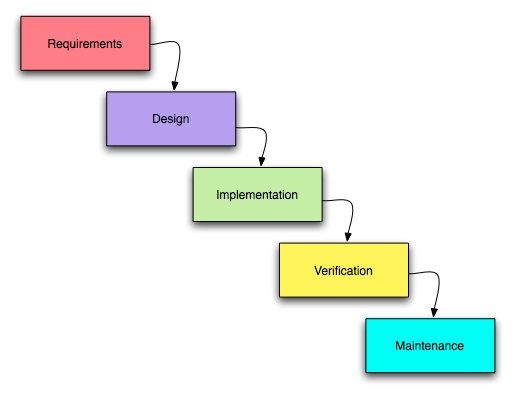
\includegraphics[width=0.5\textwidth]{Images/development_method_waterfall_model.png}
	\caption{Waterfall model}
	\label{Waterfall}
\end{figure}

The waterfall model shows a process, where developers are to follow these phases in order:
\begin{enumerate}
\item Requirements specification (Requirements analysis)
\item Software design
\item Implementation and Integration
\item Testing (or Validation)
\item Deployment (or Installation)
\item Maintenance
\end{enumerate}

\begin{figure}[h]
	\centering
	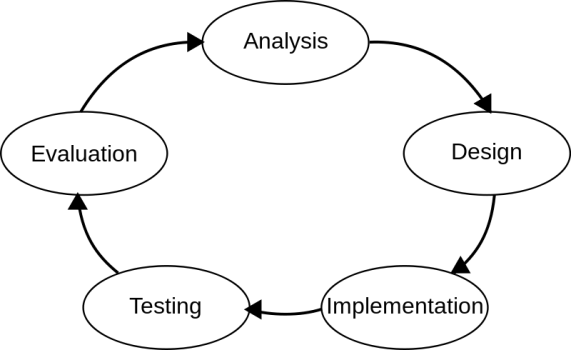
\includegraphics[width=0.5\textwidth]{Images/development_method_software_development_cycle.png}
	\caption{Software Development cycle l}
	\label{cyclel}
\end{figure}



Software Development cycle 